\documentclass{SICNU_Experiment}
\usepackage{pdfpages,tikz,amsmath,IEEEtrantools,graphicx}
\usepackage{afterpage}
\reportsetup{
  student-name    = {王小美},
  student-id      = {12345678},
  college         = {物电},
  grade           = {1807级},
  class           = {4班},
  group-number    = {3},
  teacher         = {沃雅妮莎},
  experiment-name = {今天嘉然吃什么\&泉此方那天说了什么和泥师的人文关怀},
  experiment-date = {2026-09-25},
  weekday         = {五},
}
\begin{document}
\makecover
《原神》的文化影响力远远超越了游戏本身。Sensor Tower数据显示，《原神》全球移动端每月收入的70\%来自海外市场。在日本市场，该作自上线以来累计收入已突破1500亿日元。发布171天后，游戏在全球移动设备上获得10亿美元收入；截至2022年5月，在Google Play和App Store上获得的流水超过30亿美元。
\begin{figure}[hb]
\centering

\includegraphics[width=4cm]{24.png}
\caption{What can I say?}
\end{figure}

在文化传播层面，《原神》走出了一条独特的道路。游戏不搞单向的文化输出，而是通过设定中国风格的璃月、欧洲风格的蒙德等面貌各异的区域，让全球玩家都能找到熟悉的文化入口，在对照中感知不同文明的独特气质。游戏中火爆海外的《神女劈观》段落，角色云堇并非对京剧人物的脸谱化复刻，而是拥有完整鲜活的人生设定，将戏服、身段、唱腔与人物命运融为一体。

在线下，米哈游连续举办了三届“原神FES”嘉年华，累计吸引逾20万人次参展。第三届FES展的用户80\%来自上海以外地区，充分体现了玩家群体的跨区域消费特征。游戏还两度与北京环球影城合作，将蒙德城一比一线下还原，打造沉浸式互动体验，专区门票提前两周即全部售罄。

《原神》的战斗系统围绕七大元素构建——风、雷、水、火、冰、草、岩。拥有「神之眼」的角色能够引导元素之力用于战斗和探险。元素反应系统是战斗策略的核心：水与火相遇触发「蒸发」，火与雷引起「超载」，雷遇水附加「感电」。

元素反应分为增幅反应与剧变反应两大类。增幅反应通过提升原伤害比例生效，受暴击、抗性等属性影响。例如火触发水蒸发时伤害倍率为1.5倍，水触发火蒸发则提升至2.0倍。剧变反应则与元素精通属性相关，包括超载、感电、超导、扩散等，各自产生不同的战斗效果。针对不同敌人，使用技能触发适当的元素效果，是制胜的关键。

随着版本更迭，游戏不断引入新的元素反应机制。在最新的7.0版本中，游戏新增了“星扩散反应”——由冰元素与风元素触发，反应后会生成自动爆炸并造成冰元素范围伤害的“星之岚”，多次触发还可使星之岚升级，强化爆炸范围与伤害。

从蒙德的风起地到璃月的绝云间，从稻妻的鸣神岛到须弥的智慧之城，从枫丹的水下世界到纳塔的燎火之原，再到如今至冬的永冬雪国，《原神》的冒险版图仍在不断拓展。这款游戏以其广阔的世界观、精妙的元素战斗系统、高品质的美术音乐呈现，以及不断进化的内容更新，持续为全球旅行者们带来新的惊喜与感动。动身吧，旅行者——真正的冒险才刚刚开始。
派蒙跟在她身后，叽叽喳喳地问着各种问题。荧没有回答，只是走出客栈，走进璃月港清晨的阳光里。

在她身后，望舒客栈的顶楼上，那杯凉透了的茶旁边，不知何时多了一朵小小的、半透明的花。

那朵花没有颜色，形状也在不断地变化，但它一直在开。
\part{课中实验操作}
\section{\Large 物理实验原始数据记录}
这是测试。\newpage
\section{\Large 实验操作过程\mdseries \normalsize（包括实验操作的关键步骤、注意事项、遇到的问题与解决方法）}
《ATRI -My Dear Moments》（中文常译作《亚托莉 -我挚爱的时光》）是一部由ANIPLEX.EXE企划发行，Front Wing与枕社联合制作的视觉小说（Galgame）。它于2020年6月发售，凭借精美的制作、动人的故事和鲜明的人物，被许多玩家称为“年轻人的第一部Galgame”。


\noindent 主要角色\\
\begin{center}
\begin{tabular}{lp{6cm}l}
\hline
角色&简介&配音\\
\hline
\hline
亚托莉 (Atri)&从海底打捞的机器人少女，情感丰富，好奇心旺盛。因长期沉睡而丧失部分记忆，口头禅是“因为我是高性能的嘛！”&赤尾光\\
\hline
斑鸠夏生 (Ikaruga Natsuki)&本作男主角，因事故失去一条腿，内心带有创伤，从都市移居到海边小镇&小野贤章（动画）\\
\hline
神白水菜萌 (Kamishiro Minamo)&夏生的青梅竹马，性格认真、纯朴，非常照顾夏生&高桥未奈美\\
\hline
野岛龙司 (Nojima Ryuji)&本地青年，体格健壮，性格正直，是镇上孩子们的老大&细谷佳正\\
\hline
凯瑟琳 (Catherine)&神秘的讨债人，实际身份不明，提出了打捞海底遗产的计划&日笠阳子\\
\hline
名波凛凛花 (Nanami Ririka)&居住在学校里的小学五年级少女&春野杏\\
\hline
\end{tabular}
\end{center}
主题与特色
\begin{itemize}
\item 核心主题：故事围绕“心”的定义展开。亚托莉虽为机器人，却拥有比人类更纯粹的情感，探讨了记忆、爱与牺牲的意义。
\item 艺术与音乐：游戏原画由ゆさの和基4\%负责，背景由わいっしゅ绘制，音乐则由松本文纪操刀，共同营造出海边小镇宁静而略带忧伤的氛围。
\item 全年龄定位：本作是一款全年龄向作品，没有露骨的成人内容，焦点完全放在剧情和情感表达上，适合更广泛的受众。
\end{itemize}
\newpage
\part{课后实验报告撰写}
\section{\Large 实验目的}
原神，启动！
\section{\Large 实验原理/设计\mdseries \normalsize（包括基本原理阐述、主要计算公式、有关电路、光路及实验装置示意图等）}
挪德卡莱，那夏镇。

霜月之子的祭坛深处，菈乌玛跪在月髓之前，双手交叠于胸口，额头几乎贴上冰冷的石面。月光从穹顶的裂隙中倾泻而下，在她银白色的长发上流淌成一条静止的河。

“咏月使大人。”侍从的声音从祭坛入口传来，带着不加掩饰的颤抖，“至冬的使团又来了。这次，是执行官亲自来的。”

菈乌玛没有抬头。她的呼吸均匀而缓慢，月髓的光芒在她合拢的眼睫上投下细碎的银斑。在那片光芒之中，她看见了一些不应该看见的东西。

命运之丝。菈乌玛从不主动去看它们，因为每一次窥视都会让她的灵魂被剥离出一层薄薄的、几乎透明的尘埃。那是灵魂的磨损，是咏月使与生俱来的诅咒，也是她与月神之间唯一的联系。但今天，那些丝线在她闭眼的黑暗中自发地浮现了出来。

它们正在断裂。

菈乌玛猛地睁开双眼。金色的瞳孔在月光中骤然收缩。

\begin{equation}
a^2 + b^2 = c^2
\end{equation}

\begin{IEEEeqnarray}{rCl}
a & = & b + c
\\
& = & d + e + f + g + h
+ i + j + k \nonumber\\
&& \negmedspace {} + l + m + n + o
\\
& = & p + q + r + s
\end{IEEEeqnarray}

“告诉至冬人，”她站起身来，苍白的衣袍在身后拖曳出一道长长的弧线，“霜月之子今天不接待任何访客。”

但至冬人并不需要她的许可。祭坛的石门在一声沉闷的轰鸣中向两侧滑开，一个身穿白色长袍的身影逆光走了进来。他戴着半张面具，面具下的嘴角挂着一丝极淡的笑意。

“咏月使，”那声音很轻，像冰层之下暗流涌动的水，“女皇陛下让我来取一件东西。不是神之心——我们暂时对霜月之子的信仰没有兴趣。我们想要的，是你看到的那些丝线。”

菈乌玛的指尖微微发凉。

行内公式$\displaystyle \int_a^b {f(x)\,\mathrm{d}x} = F(b) - F(a)$测试。

“……你们在收集神之心。”她说。

“不止。”执行官向前迈了一步，月髓的光芒在他身后拉出一道极长的影子，那影子的边缘在石面上悄然扭曲，仿佛有自己的意志，“神之心是第三降临者的遗骨，是‘理’的碎片。但女皇陛下需要的不只是‘理’。她需要‘命运’本身。”

他抬起手，掌心悬浮着一枚暗银色的齿轮，齿轮的每一道齿牙上都刻着密密麻麻的、肉眼几乎无法辨认的铭文。

“天理的‘神圣规划’，”执行官说，“本质是一台织机。它只织一条线，而把其他所有线的可能全部剪断。被剪断的线不会消失，它们会坠入深渊，变成恨意。”

菈乌玛知道这一点。所有的咏月使都知道这一点。但没有人敢说出来。

“所以女皇陛下要做什么？”

“重置织机。”执行官收回齿轮，语气平淡得像在谈论明天的天气，“让所有的线都能被织入。让‘未发生的命运’不再成为恨意。至冬不打算毁灭天理——至冬打算修复它。”

菈乌玛沉默了很久。月光在她脸上缓慢地移动，像一只犹豫的手。

“你不能相信他们。”一个声音从祭坛的阴影中传来。

旅行者从侧廊走出，身后跟着派蒙。荧的手按在剑柄上，金色的眼睛盯着执行官，瞳孔深处有一丝几乎不可见的疲惫。那是走过七个国家、见过七个神、始终在寻找一个答案的人的眼神。

\begin{minipage}{4cm}


\includegraphics[height=3cm]{nahida.png}

\end{minipage}

“菈乌玛，”荧说，“他们说的‘重置织机’，代价是什么？”

菈乌玛闭上了眼睛。

在她闭眼的黑暗中，命运之丝再次浮现，而这一次她看见了更多的细节，每条丝线上都系着一个人。有的丝线正在发出微弱的、痛苦的颤光，仿佛被什么东西从远端拉扯。那些颤动的丝线，全都指向同一个方向。

至冬。

“代价是，”菈乌玛睁开眼，声音轻得像一片即将落地的霜，“所有被织入‘新织机’的丝线，都需要一个锚点。一个活着的、承载着那条命运的人。如果那条命运从未发生过……那个人，就不需要存在了。”

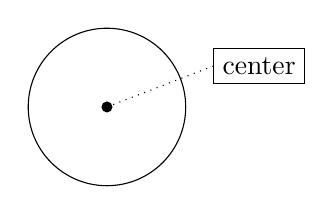
\begin{tikzpicture}
\draw (0,0) circle[radius=1];
\fill (0,0) circle[radius=2pt];
\node[draw] (P) at (15:2) {center};
\draw[dotted] (0,0) -- (P.west);
\end{tikzpicture}
祭坛安静了下来。

执行官面具下的笑意没有消失，但也没有加深。

“所以你们要做的，”荧缓缓拔出剑，剑锋在月光中映出一道冷白的光，“是杀掉所有‘未发生’的人。”

“不。”执行官摇头，“是让他们‘不需要存在’。这两者之间，有很大的区别。”

他转身走向祭坛出口，白袍在石面上拂过，像一场正在退去的雪。

“女皇陛下不着急，”他在石门边缘停下，没有回头，“但深渊不等人。你们很快就会发现，比起天理的暴政，虚无才是真正的敌人。”

石门合拢。月光重新变得完整。

菈乌玛跪坐在地，双手捂住了脸。
\newpage
\section{\Large 数据处理及实验结果\mdseries \normalsize（包括具体计算过程、平均值和不确定度等的计算公式以及最后的实验结果）}
游戏的故事发生在一片被称作「提瓦特」的广袤大陆上。这里是七神统治、七种元素交汇的世界，无数生灵繁衍聚集于此，天地万象蕴含其间。在遥远的过去，人们藉由对神灵的信仰，获赐了驱动元素的力量，得以在荒野中筑起家园。然而五百年前，古国的覆灭却使得天地变异，如今席卷大陆的灾难虽然已经停息，和平却仍未如期光临。

玩家在游戏中扮演一位从世界之外漂流而来的旅行者。故事的开端，一对旅行中的双子降临这片大地，但血亲被陌生的神灵带走，而玩家自身也被神封印，陷入沉眠。再度醒来时，天地间风景已变。作为故事的主角，玩家将在这片广阔的世界中自由旅行、结识同伴、寻找掌控尘世元素的七神，踏上寻回血亲之路，直到与分离的血亲重聚，在终点见证一切旅途的沉淀。
\newpage
\section{\Large 问题讨论与误差分析\mdseries \normalsize（包括回答思考题、误差分析、对实验的改进意见或独到见解以及实验的应用前景等）}
我是山里灵活的狗。
这是测试，原神。

故事设定在人类与兽人共存的现代都市。主角尼古喵喵（本名佐藤尼古子）是一只重度烟瘾的猫娘兽人，她毫无生活自律，沉迷烟草、拒绝成长。

她的日常围绕着“攒钱买烟”展开，房间堆满烟蒂和垃圾，缺乏基本的伦理与卫生观念，会乱扔烟头甚至对人吐口水。幸运（或不幸）的是，她身边有管家型的妹妹猫和好友嗑药猫的纵容，让她能继续沉溺于这种散漫荒诞的生活。

《尼古喵喵》并非一部传统意义上的治愈系猫娘动画。它用粗粝直白的方式，刻画了一个被成瘾问题困扰的“废柴”兽人形象。如果你对黑色幽默、社会观察以及带有荒诞感的作品感兴趣，它可能会带来一种截然不同的观看体验。
\end{document}